\subsection{\label{subsec:FZV3}Frage 3}
\textbf{\textit{Berechnen Sie den theoretischen Durchmesser des THz-Strahls bei bestmöglicher
Fokussierung in Abhängigkeit der Frequenz (0,5 - 3 THz) und vergleichen Sie dies
mit dem Fokusdurchmesser eines 1550 nm Strahls. Nehmen Sie an, dass beide
Strahlen von einer Linse mit Brennweite f = 25 mm fokussiert werden und beide
Eingangsstrahlen einen Durchmesser von D = 20 mm besitzen.}}\\
$\rightarrow$Der theoretisch erreichbare Durchmesser eines fokussierten THz-Strahls ist durch 
die physikalische Auflösungsgrenze (Abbe-Limit) begrenzt. Für die erreichbare 
Auflösung und damit dem minimalen Durchmesser des fokussierten Strahls $d$ gilt
\begin{equation}
    d = \frac{\lambda}{n\sin(\alpha)} = \frac{c}{\nu n\sin(\alpha)}.
\end{equation} 
Hierbei beschreibt $n$ den Brechungsindex zwischen Präparat und Linse ($n_{\text{Luft}}=1$), $c$ ist die Lichtgeschwindigkeit und 
$\alpha$ gibt den halben Öffnungswinkel an (siehe Abb.~\ref{fig:abbe}). 
\begin{figure}[h!]
    \centering
    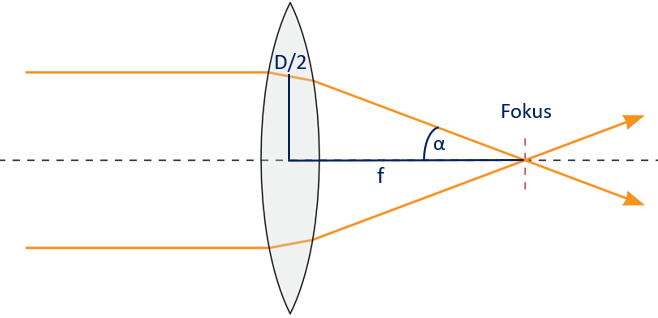
\includegraphics[width=0.7\textwidth]{Linse.png}
    \caption{\label{fig:abbe}Schematische Darstellung der Fokussierung eines Lichtstrahls des Durchmessers $D$
    durch eine Sammellinse der Brennweite $f$. Der halbe Öffnungswinkel $\alpha$ lässt sich 
    über geometrische Überlegungen berechnen.}
\end{figure}\FloatBarrier
Der Sinus dieses Winkels lässt sich über die Trigonometrischen Gleichungen berechnen, womit 
eine Bestimmungsgleichung des theoretischen Fokusdurchmessers folgt, die reziprok proportional zur 
Frequenz des Lichtstrahls ist
\begin{align}
    n\sin(\alpha) &= \frac{\text{Gegenkathete}}{\text{Hypothenuse}} = \frac{D/2}{\sqrt{(D/2)^{2} + (f)^{2}}} \\
    \Rightarrow\Aboxed{d &= \frac{c}{\nu}\frac{\sqrt{(D/2)^{2} + (f)^{2}}}{D/2}}.
\end{align}
Hieraus erkennt man, dass die Fokussierung mit steigender Frequenz besser wird.
Folgende Werte gelten für die fokussierten Strahlendruchmesser
\begin{equation}
    \fbox{$d_{\nu=0,5\,\si{THz}} \approx ABC\,\si{mm}\hspace{1cm}d_{\nu=3\,\si{THz}} \approx ABC\,\si{mm}
    \hspace{1cm}d_{\lambda=1550\,\si{nm}} \approx ABC\,\si{\mu m}$}.
\end{equation}
